\documentclass[conference]{IEEEtran}
\pagestyle{plain}
\usepackage[pdftex]{graphicx}
\graphicspath{{../pdf/}{../jpeg/}}
\DeclareGraphicsExtensions{.pdf,.jpeg,.png}
\usepackage{changepage}
\usepackage[utf8]{inputenc}
\usepackage[T1]{fontenc}
\usepackage{matlab-prettifier}
\usepackage{circuitikz, siunitx}
\usepackage[cmex10]{amsmath}
\usepackage{mathabx}
\usepackage{algorithmic}
\usepackage{float}
\usepackage{array}
\usepackage{mdwmath}
\usepackage{mdwtab}
\usepackage{eqparbox}
\usepackage{url}
\usepackage{makecell}
\usepackage{tikz}
\usepackage{xcolor}
\usepackage{pgfplots}
\IEEEoverridecommandlockouts
\IEEEpeerreviewmaketitle

\pgfplotsset{compat=1.18} 
\usetikzlibrary{shapes.geometric, arrows, arrows.meta, positioning, patterns}

\tikzstyle{startstop} = [rectangle, rounded corners, 
minimum width=3cm, 
minimum height=1cm,
text centered, 
draw=black]

\tikzstyle{io} = [trapezium, 
trapezium stretches=true,
trapezium left angle=70, 
trapezium right angle=110, 
minimum width=3cm, 
minimum height=1cm, text centered, 
draw=black]

\tikzstyle{process} = [rectangle, 
minimum width=3cm, 
minimum height=1cm, 
text centered, 
text width=3cm, 
draw=black]

\tikzstyle{decision} = [diamond, 
minimum width=3cm, 
minimum height=1cm, 
text centered, 
draw=black]

\tikzstyle{arrow} = [thick,->,>=stealth]
\tikzstyle{invarrow} = [thick,<-,>=stealth]
        
\begin{document}

\title{Sistema de Adquisición y Procesamiento de Datos para la Caracterización $V-I$ y Estimación Térmica en Diodos}

\author{
    \authorblockN{
        B. Castro [1], A. Machado [2], L. Pineda [3], M. Rodríguez [4], J. Romero [5]
    }
    \authorblockA{
        \textit{Universidad de los Llanos} \\
        \textit{Villavicencio, Colombia} \\ 
        \begin{tabular}{c}
            \small \texttt{[1] 161004905 - bacastro@unillanos.edu.co}\\
            \small \texttt{[2] 161004922 - ammachado@unillanos.edu.co}\\
            \small \texttt{[3] 161004933 - lapineda.sibo@unillanos.edu.co}\\
            \small \texttt{[4] 161004834 - marodriguez.payares@unillanos.edu.co}\\
            \small \texttt{[5] 161004937 - jfromero.esquivel@unillanos.edu.co}\\
        \end{tabular}
    }
}
\IEEEaftertitletext{\vspace{-1\baselineskip}}
\maketitle

\renewcommand\abstractname{Resumen}\begin{abstract}
Este artículo presenta el diseño e implementación de un sistema automatizado para la caracterización eléctrica y estimación térmica de diodos mediante el análisis de su curva de voltaje-corriente ($V-I$). Se desarrolló un sistema de adquisición de datos (DAQ) determinista basado en el microcontrolador ESP32, diseñado para capturar la respuesta del dispositivo bajo una excitación senoidal de \SI{1}{\hertz}. Para garantizar la integridad de las mediciones, se implementó una etapa de acondicionamiento activo que adapta las señales bipolares del circuito a los rangos unipolares del convertidor analógico-digital (ADC). Los datos capturados son transmitidos vía comunicación serial de alta velocidad hacia una estación de trabajo, donde un algoritmo en Python filtra y procesa la información aplicando la ecuación de Shockley. Mediante técnicas secuenciales de regresión por mínimos cuadrados y optimización no lineal (algoritmo de Levenberg-Marquardt), se extrae de manera robusta el factor de idealidad ($\eta$) a temperatura controlada. Posteriormente, utilizando el factor extraído como constante estructural, se invierte el modelo matemático para estimar la temperatura absoluta ($T$) del semiconductor bajo diferentes condiciones de operación. La metodología propuesta demuestra alta precisión y viabilidad para evaluar el comportamiento físico de los semiconductores y su aplicación como sensores térmicos.
\end{abstract}

\renewcommand\IEEEkeywordsname{Palabras clave}\begin{keywords}
Acondicionamiento de señales, Adquisición de datos, Ecuación de Shockley, ESP32, Factor de idealidad, Regresión no lineal, Termometría de diodo.
\end{keywords}

\section{Introducción}
\label{sec:introduccion}

\IEEEPARstart{E}{l} estudio de los dispositivos semiconductores es un pilar de la electrónica moderna. El diodo de unión p-n, como componente fundamental, presenta un comportamiento eléctrico no lineal que depende estrictamente de sus características físicas y de las condiciones térmicas de operación \cite{boylestad_dispositivos, neamen_fisica_semiconductores}. Comprender la relación entre la corriente y el voltaje (curva $V-I$) es esencial para el modelado preciso de dispositivos más complejos y para el análisis de fenómenos como la inyección y recombinación de portadores de carga \cite{karg1997light, wilson1970comparison}.

Teóricamente, el comportamiento de un diodo bajo polarización se describe mediante la ecuación del diodo de Shockley \cite{vliet1980shockley, musolino2016modified}, la cual establece que la corriente a través del dispositivo ($I_D$) está dada por:
\begin{equation}
    I_D = I_S \left( \exp  \left( {\frac{q V_D}{\eta k T}}\right) - 1 \right)
    \label{eq:shockley}
\end{equation}
donde $I_S$ es la corriente de saturación inversa, $q$ es la carga del electrón, $k$ es la constante de Boltzmann, $\eta$ es el factor de idealidad (que ajusta las desviaciones del modelo ideal) y $T$ es la temperatura absoluta de la unión en Kelvin. 

La temperatura de la unión del semiconductor ($T$) es un parámetro dinámico y crítico, ya que el auto-calentamiento y las variaciones térmicas del entorno modifican significativamente las propiedades eléctricas del material \cite{oh2017junction, long2012numerical}. De hecho, el análisis de las características de voltaje directo y corriente inversa es una técnica ampliamente validada en la literatura para determinar de forma indirecta la temperatura de la unión en diversos dispositivos, desde rectificadores básicos hasta diodos emisores de luz \cite{wu2013junction, han2014influence}. 

El presente laboratorio tiene como objetivo principal caracterizar la respuesta térmica de un diodo mediante la captura de sus curvas de voltaje y corriente a distintas temperaturas. Para ello, se implementó un sistema de adquisición de datos de alta velocidad basado en el microcontrolador ESP32. El procedimiento experimental consta de dos etapas fundamentales: en primer lugar, se realiza una calibración mediante la toma de datos a una temperatura ambiente conocida para calcular, a través de regresión, el factor de idealidad empírico ($\eta$) del diodo; en segundo lugar, asumiendo la invariabilidad de dicho parámetro físico en el rango de prueba, se utiliza la pendiente de nuevas regresiones obtenidas al aplicar calor para estimar la temperatura real de la unión ($T$). Mediante este enfoque, se valida la aplicabilidad de los modelos matemáticos de semiconductores para la metrología térmica.

\vspace{3mm}
\noindent Disponibilidad del Código: Para fines de reproducibilidad y consulta técnica, los archivos fuente del firmware (\texttt{.ino}), los scripts de captura y el programa de procesamiento de datos (\texttt{.py}) presentados en este artículo se encuentran alojados en el repositorio público: \url{https://github.com/Nocudo/Lab-3}.
\vspace{3mm}

\section{Metodología}
\label{sec:metodologia}

En esta sección se detalla el diseño del hardware de adquisición y el protocolo de procesamiento de señales utilizado para caracterizar la respuesta térmica del diodo bajo prueba.

\subsection{Circuito de Caracterización del Diodo}
\label{subsec:circuito_diodo}

Para obtener la relación voltaje-corriente ($V-I$) del dispositivo, se implementó un circuito de prueba alimentado por una fuente de tensión senoidal $V_s$ con una amplitud de \SI{6}{\volt} pico-pico y una frecuencia de \SI{1}{\hertz}, tal como se muestra en la Fig. \ref{fig:circuito_esquematico}. El circuito consiste en una red serie conformada por una resistencia de precisión $R_s = \SI{217}{\ohm}$ y un diodo bajo estudio.

El monitoreo de las variables físicas se realiza en dos puntos estratégicos:
\begin{itemize}
    \item Nodo $V_A$: Registra la tensión total suministrada por el generador.
    \item Nodo $V_B$: Registra la caída de tensión en el diodo, referenciada a la resistencia de carga.
\end{itemize}

De acuerdo con la Ley de Ohm y las leyes de Kirchhoff \cite{boylestad_dispositivos}, la corriente que circula por el diodo ($i_D$) y el voltaje en sus terminales ($V_D$) se determinan mediante:
\begin{equation}
    V_D = V_B
\end{equation}
\begin{equation}
    i_D = \frac{V_A - V_B}{R_s}
\end{equation}

\begin{figure}[htbp]
    \centering
    \begin{circuitikz}[american voltages, scale=0.7, transform shape]
        % Circuito principal
        \draw
            (0,0) to [vsourcesin, l=$V_s$, a=$\begin{array}{l} V_{pp}\text{ = } \SI{6}{\volt} \\ f \text{ = }\SI{1}{\hertz}
            \end{array}$] ++(0,3) coordinate (VA)
            node[anchor=south east]{$V_A$}
            to [R, l=$R_s$, a=$\SI{217}{\ohm}$, *-*, i=$i_D$] ++(5,0) coordinate (VB)
            node[anchor=south west]{$V_B$}
            to [diode={light emitting}, l=$D$] ++(0,-3)
            |- (0,0)
            node[ground] {};
            
        % Bloque de acondicionamiento para Va
        \draw (VA) to[short] (0, 4) 
            node[draw, rectangle, minimum width=2.8cm, minimum height=1.2cm, anchor=south, align=center] (CondA) {Circuito de \\ Acondicionamiento};
        \draw (CondA.north) to [short, -o] ++(0,0.6) node[above] {GPIO 34};

        % Bloque de acondicionamiento para Vb
        \draw (VB) to[short] (5, 4) 
            node[draw, rectangle, minimum width=2.8cm, minimum height=1.2cm, anchor=south, align=center] (CondB) {Circuito de \\ Acondicionamiento};
        \draw (CondB.north) to [short, -o] ++(0,0.6) node[above] {GPIO 35};

    \end{circuitikz}
    \caption{Circuito propuesto con etapas de acondicionamiento de señal.}
    \label{fig:circuito_esquematico}
\end{figure}


\subsection{Acondicionamiento de Señales para el ADC}
\label{subsec:acondicionamiento}

Dado que las señales $V_A$ y $V_B$ presentan componentes negativas (rango de \SI{-3}{\volt} a \SI{3}{\volt}) y el ADC de la ESP32 solo admite tensiones unipolares entre \SI{0}{\volt} y \SI{3.3}{\volt}, se diseñó una etapa de acondicionamiento activa basada en amplificadores operacionales (Fig. \ref{fig:circuito_acondicionamiento}).

\subsubsection{Etapa de Suma y Desplazamiento (Offset)}
Se utilizó un amplificador operacional (U1) en configuración sumadora inversora. Las entradas del sumador son la señal bajo medición ($V_{in}$) y una referencia de tensión de \SI{-3}{\volt}, ambas acopladas mediante resistencias de $R_2 = R_3 = \SI{10}{\kilo\ohm}$. Con una resistencia de retroalimentación $R_4 = \SI{10}{\kilo\ohm}$, la salida del operacional entrega una señal desplazada y positiva:
\begin{equation}
    V_{op} = -\left( \frac{R_4}{R_2}V_{in} + \frac{R_4}{R_3}(-3) \right) = 3 - V_{in}
\end{equation}
Para una entrada de $\pm\SI{3}{\volt}$, esta etapa genera un rango de salida de \SI{0}{\volt} a \SI{6}{\volt}.

\subsubsection{Etapa de División de Tensión}
Para ajustar el nivel a los límites del microcontrolador, se integró un divisor resistivo a la salida del operacional compuesto por $R_5 = R_6 = \SI{10}{\kilo\ohm}$. Esto atenúa la señal a la mitad:

\begin{equation}
   V_{out}=\left( \frac{R_6}{R_5 + R_6} \right) V_{op} =  \frac{3-V_{in}}{2}
\end{equation}

El resultado es un rango final de \SI{0}{\volt} a \SI{3}{\volt}, óptimo para la resolución del ADC \cite{dunn_instrumentacion}. La señal acondicionada ($V_{out}$) se conecta a los pines GPIO 34 y 35 de la ESP32 para su digitalización.

\begin{figure}[htbp]
    \centering
    \begin{circuitikz}[scale=0.7, transform shape]
        
        % Entrada -3V y R3
        \draw (0,6) node[anchor=east] {-3V} to[R, l=$R_3$, a=10k$\Omega$, *-*] (3,6) coordinate(junc2);

        % Entrada Vin y R2
        \draw (0,4.5) node[anchor=east] {$V_{in}$} to[R, l=$R_2$, a=10k$\Omega$, *-*] (3,4.5) coordinate(junc1);

        % Amplificador Operacional U1 (orientación por defecto, hacia la derecha)
        \draw (5,4) node[op amp] (U1) {};
        \node[above] at (5, 4.8) {U1};
        \node[below] at (5, 3.2) {OPAMP};

        % Conexiones de entrada del OpAmp
        \draw (junc1) -- (U1.-);
        \draw (U1.+) -- ++(0,-0.5) node[ground]{};

        % Línea vertical uniendo la rama de -3V con el pin inversor
        \draw (junc1) -- (junc2);

        % Resistencia de retroalimentación R4 y cierre del lazo
        \draw (junc2) to[R, l=$R_4$, a=10k$\Omega$, -] (7.5,6) -- (7.5,4) coordinate(out_div);
        \draw (U1.out) -- (out_div);

        % Divisor de tensión a la salida
        \draw (out_div) to[R, l_=$R_5$, a^=10k$\Omega$, *-*] ++(0,-3) coordinate(esp_node);
        \draw (esp_node) to[R, l_=$R_6$, a^=10k$\Omega$] ++(0,-3) node[ground]{};

        % Etiqueta de salida Vout
        \draw (esp_node) to[short, -o] ++(1.2, 0) node[anchor=west]{$V_{out}$};
        
    \end{circuitikz}
    \caption{Esquema de conexión detallado para el acondicionamiento de señal.}
    \label{fig:circuito_acondicionamiento}
\end{figure}

\subsection{Desarrollo del Firmware y Lógica de Adquisición}
\label{subsec:firmware}

El control del sistema de adquisición de datos (DAQ) reside en un firmware desarrollado para la plataforma ESP32, cuya función es garantizar un muestreo de alta velocidad y baja latencia. El programa opera bajo un esquema de "petición-respuesta", donde el microcontrolador permanece en estado de reposo hasta detectar el comando de sincronización vía serial (ver Fig. \ref{fig:flow_esp32}).

\begin{figure}[htbp]
    \centering
    \resizebox{0.7\columnwidth}{!}{
    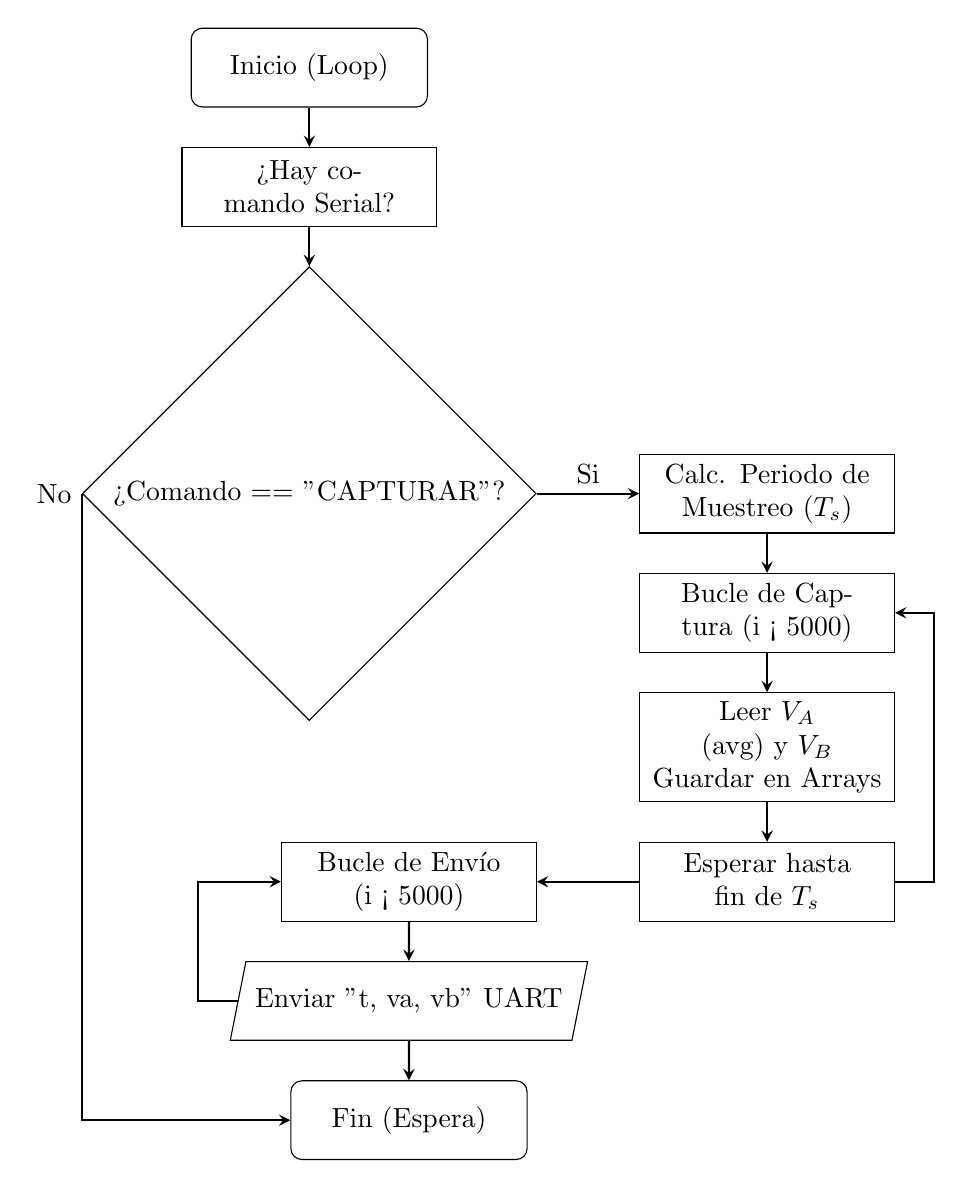
\begin{tikzpicture}[node distance=0.5cm, auto]
        
        % --- Definición de nodos ---
        \node (start) [startstop] {Inicio (Loop)};
        \node (serial) [process, below=of start] {¿Hay comando Serial?};
        \node (dec_cmd) [decision, below=of serial] {¿Comando == "CAPTURAR"?};
        \node (init) [process, right=of dec_cmd, xshift=0.8cm] {Calc. Periodo de Muestreo ($T_s$)};
        
        \node (loop_cap) [process, below=of init] {Bucle de Captura (i < 5000)};
        \node (adc) [process, below=of loop_cap] {Leer $V_A$ (avg) y $V_B$ \\ Guardar en Arrays};
        \node (wait) [process, below=of adc] {Esperar hasta fin de $T_s$};
        
        \node (loop_send) [process, left=of wait, xshift=-0.8cm] {Bucle de Envío (i < 5000)};
        \node (proc_send) [io, below=of loop_send] {Enviar "t, va, vb" UART};
        
        \node (stop) [startstop, below=of proc_send] {Fin (Espera)};

        % --- Conexiones ---
        \draw [arrow] (start) -- (serial);
        \draw [arrow] (serial) -- (dec_cmd);
        
        \draw [arrow] (dec_cmd) -- node[anchor=south] {Si} (init);
        \draw [arrow] (dec_cmd.west) node[anchor=east] {No} |-  (stop);
        
        \draw [arrow] (init) -- (loop_cap);
        \draw [arrow] (loop_cap) -- (adc);
        \draw [arrow] (adc) -- (wait);
        
        \draw [arrow] (wait.west) -- (loop_send.east);
        \draw [arrow] (loop_send) -- (proc_send);
        \draw [arrow] (proc_send) -- (stop);

        % Retorno de bucles (conceptual)
        \draw [arrow] (wait.east) -- ++(0.5,0) |- (loop_cap.east);
        \draw [arrow] (proc_send.west) -- ++(-0.5,0) |- (loop_send.west);

    \end{tikzpicture}
    }
    \caption{Diagrama de flujo del firmware de adquisición de datos en la ESP32 (\texttt{captura.ino}).}
    \label{fig:flow_esp32}
\end{figure}

\subsubsection{Determinación del Periodo de Muestreo}
Para reconstruir fielmente la dinámica del diodo, el firmware calcula dinámicamente el tiempo entre muestras ($T_s$) en microsegundos. Este cálculo se basa en la frecuencia de la señal de excitación ($f_s = \SI{1}{\hertz}$), el número de periodos de la onda que se desean capturar ($N_p = 2$) y la resolución temporal definida por el total de muestras ($N_{samples} = 5000$). La ecuación implementada en el código es:
\begin{equation}
    T_{\mu s} = \frac{1 \times 10^6 N_p}{f_s N_{samples}}
    \label{eq:periodo_muestreo}
\end{equation}
Con los parámetros establecidos, el sistema asegura un intervalo de muestreo constante de \SI{400}{\micro\second}, lo que permite una captura detallada de los ciclos de conducción y bloqueo del componente.

\subsubsection{Algoritmo de Captura y Reducción de Ruido}
Una vez iniciado el proceso, el firmware ejecuta un bucle de alta prioridad. Para mejorar la integridad de la señal en el ánodo ($V_A$), la cual es más susceptible a transitorios de conmutación, se implementó una técnica de sobremuestreo y promediado aritmético. El valor almacenado para cada instante $i$ se define como:
\begin{equation}
    V_{A,i} = \frac{ADC(34)_{read1} + ADC(34)_{read2}}{2}
\end{equation}
Inmediatamente después, se realiza la lectura simple de la señal en el cátodo ($V_B$) a través del pin GPIO 35. Esta secuencia minimiza el desfase temporal entre las dos lecturas necesarias para calcular la corriente instantánea.

\subsubsection{Control de Jitter y Sincronización}
Para mitigar el error de temporización acumulado (jitter), el firmware emplea un control de tiempo real basado en el reloj interno del sistema. En cada iteración, se calcula el tiempo de procesamiento consumido por las lecturas analógicas y la escritura en memoria ($t_{proc}$):
\begin{equation}
    t_{delay} = T_{\mu s} - (\text{micros}_{final} - \text{micros}_{inicio})
\end{equation}
Si el tiempo de procesamiento es menor al periodo objetivo ($T_{\mu s} > t_{proc}$), el microcontrolador aplica un retardo compensatorio mediante la función \texttt{delayMicroseconds()}. Esta lógica garantiza que la base de tiempo de los archivos CSV generados sea lineal y coherente, permitiendo que el script de procesamiento en Python realice transformaciones de dominio (como la integración o derivación) sin errores de escala temporal.

\subsubsection{Transmisión y Almacenamiento}
Tras completar la ráfaga de \num{5000} muestras, los datos almacenados en los arreglos de memoria se transmiten de forma masiva hacia la estación de trabajo a una tasa de \num{921600} baudios. El formato de salida es una trama de texto delimitada por comas (CSV) con la estructura \texttt{[Tiempo, Va, Vb]}, facilitando su lectura directa mediante la librería \textit{pandas} en la etapa de análisis de resultados.

\subsection{Interfaz de Computador y Almacenamiento de Datos}
\label{subsec:interfaz_python}

El enlace entre el hardware de adquisición (ESP32) y la etapa de análisis estadístico se gestionó mediante un script desarrollado en Python (\texttt{captura.py}). Este programa actúa como la estación maestra, controlando el inicio de la captura, garantizando la integridad de las tramas de datos y consolidando la información en formatos estandarizados para su posterior procesamiento (ver Fig. \ref{fig:flow_python}).

\begin{figure}[htbp]
    \centering
    \resizebox{0.7\columnwidth}{!}{
    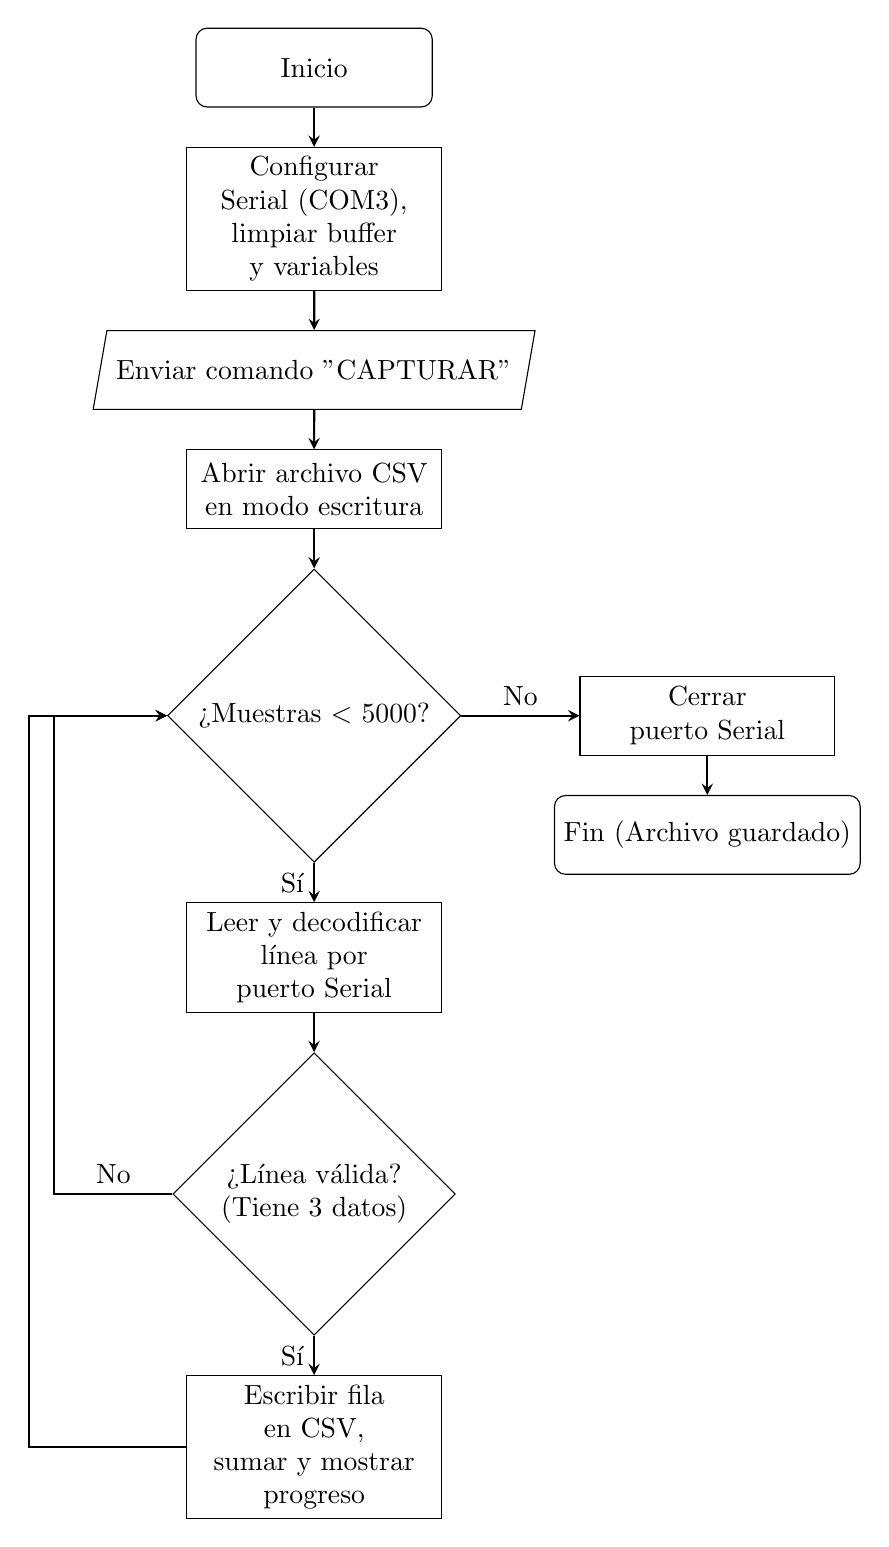
\begin{tikzpicture}[node distance=0.5cm, auto]
        
        % --- Definición de nodos ---
        \node (start) [startstop] {Inicio};
        \node (init) [process, below=of start, align=center] {Configurar Serial (COM3), \\ limpiar buffer y variables};
        \node (send) [io, below=of init] {Enviar comando "CAPTURAR"};
        \node (open) [process, below=of send, align=center] {Abrir archivo CSV \\ en modo escritura};
        
        \node (loop) [decision, below=of open] {¿Muestras $<$ 5000?};
        
        \node (read) [process, below=of loop, align=center] {Leer y decodificar \\ línea por puerto Serial};
        \node (valid) [decision, below=of read, align=center] {¿Línea válida? \\ (Tiene 3 datos)};
        \node (save) [process, below=of valid, align=center] {Escribir fila en CSV, \\ sumar y mostrar progreso};
        
        \node (close) [process, right=of loop, xshift=1cm] {Cerrar puerto Serial};
        \node (stop) [startstop, below=of close] {Fin (Archivo guardado)};

        % --- Conexiones ---
        \draw [arrow] (start) -- (init);
        \draw [arrow] (init) -- (send);
        \draw [arrow] (send) -- (open);
        \draw [arrow] (open) -- (loop);
        
        % Flujo principal del bucle
        \draw [arrow] (loop) -- node[anchor=east] {Sí} (read);
        \draw [arrow] (read) -- (valid);
        \draw [arrow] (valid) -- node[anchor=east] {Sí} (save);
        
        % Salida del bucle
        \draw [arrow] (loop) -- node[anchor=south] {No} (close);
        \draw [arrow] (close) -- (stop);

        % --- Retornos de bucle ---
        % Retorno si los datos se guardaron correctamente
        \draw [arrow] (save.west) -- ++(-2,0) |- (loop.west);
        % Retorno si la línea está vacía o incompleta (ignorar y volver a leer)
        \draw [arrow] (valid.west) -- node[anchor=south] {No} ++(-1.5,0) |- (loop.west);

    \end{tikzpicture}
    }
    \caption{Diagrama de flujo del script de Python para la adquisición y guardado de datos (\texttt{captura.py}).}
    \label{fig:flow_python}
\end{figure}

\subsubsection{Sincronización y Control Serial}
La comunicación con el microcontrolador se estableció empleando la librería \texttt{pyserial}, configurando un puerto serial virtual (COM) a una tasa de transferencia de \num{921600} baudios. Al inicializar la conexión, el script impone un retardo de seguridad de \SI{2}{\second} para permitir el reinicio automático (\textit{auto-reset}) de la ESP32 tras abrir el puerto. Seguidamente, se limpia el búfer de entrada (\texttt{reset\_input\_buffer()}) para descartar cualquier ruido o dato residual en la línea antes de enviar el comando de activación (\texttt{"CAPTURAR"}).

\subsubsection{Validación y Estructuración de la Trama}
Una vez que el microcontrolador responde y comienza a transmitir la ráfaga de mediciones, el script ingresa en un ciclo de recepción estrictamente acotado a la cantidad de muestras objetivo ($N = 5000$). Para evitar la corrupción del archivo final por errores de transmisión, cada línea de texto recibida se somete a un proceso de filtrado y validación:

\begin{enumerate}
    \item Decodificación: La secuencia de bytes se decodifica al estándar UTF-8, ignorando caracteres erróneos producto de posibles interferencias electromagnéticas en la línea UART.
    \item Limpieza y Fragmentación: Se eliminan los saltos de línea o espacios en blanco residuales (\texttt{strip()}) y se divide la cadena utilizando la coma como carácter delimitador.
    \item Control de Longitud: El sistema verifica rigurosamente que la tupla extraída contenga exactamente tres elementos correspondientes a la estructura definida: $[t, V_A, V_B]$. 
\end{enumerate}

\subsubsection{Generación de Archivos CSV}
Las tramas que superan la validación estructural se registran secuencialmente en el disco de la estación de trabajo utilizando la librería nativa \texttt{csv}. Los archivos resultantes son nombrados de acuerdo a la temperatura de ensayo correspondiente (por ejemplo, \texttt{25°C.CSV}, \texttt{40°C.CSV}), creando un repositorio de datos ordenado. Este formato delimitado por comas resulta ideal para importar la información de forma directa a estructuras \textit{DataFrame} de la librería \textit{pandas} durante la fase posterior de análisis y regresión lineal por mínimos cuadrados.

\subsection{Metodología de Ajuste de Curva y Cálculo de Errores}
\label{subsec:metodologia_ajuste}

Para extraer empíricamente el factor de idealidad ($\eta$) a partir de los datos experimentales, se utilizó la Ecuación del Diodo (Shockley) reescrita y adaptada para el ajuste. Esta variante incorpora un término constante $C$, el cual incluye efectos de la resistencia en serie y posibles compensaciones de corriente de offset del instrumental. El modelo matemático base se define como:
\begin{equation}
    I = A \left( \exp(B V) - 1 \right) + C
    \label{eq:ajuste_base}
\end{equation}
donde el parámetro $A \approx I_0$ y el coeficiente del exponente se define como $B \approx \frac{q}{\eta k T}$. Una vez determinado el coeficiente $B$, el factor de idealidad se puede despejar directamente mediante:
\begin{equation}
    \eta = \frac{q}{k B T}
    \label{eq:factor_idealidad_b}
\end{equation}

Dada la fuerte no linealidad de la Ecuación \ref{eq:ajuste_base}, la extracción paramétrica se ejecutó en dos fases metodológicas distintas implementadas a través de algoritmos computacionales:

\subsubsection{Ajuste Emergencial (Aproximación Lineal)}
En la región de alta polarización directa, caracterizada por la condición $V \gg \frac{\eta k T}{q}$, el modelo exponencial se puede simplificar despreciando el término unitario. Esto permite linealizar la ecuación aplicando logaritmos naturales:
\begin{equation}
    \ln\left( \frac{I - C}{A} + 1 \right) \approx B V
\end{equation}
El cálculo se implementó mediante la función \texttt{regresion\_emergencial}, la cual ejecuta una aproximación por mínimos cuadrados ponderados sobre este espacio logarítmico transformado. El algoritmo halla la pendiente del sistema ($B$) forzando su intersección en el origen. Aunque este ajuste es aproximado, su propósito principal es proporcionar un valor de semilla altamente confiable y cercano a la solución real para la etapa de optimización posterior.

\subsubsection{Ajuste No Emergencial (Ajuste No Lineal)}
Para incorporar el comportamiento físico en toda la curva de polarización y maximizar la precisión, se utilizó la función \texttt{regresion\_no\_emergencial}. Este enfoque utiliza la forma completa del modelo del diodo descrita en la Ecuación \ref{eq:ajuste_base} a través del algoritmo de Levenberg-Marquardt.

Este método numérico es altamente robusto ya que combina la convergencia rápida del método de Gauss-Newton cerca del mínimo con la estabilidad direccional del descenso de gradiente. Al inicializar el algoritmo con el coeficiente $B$ obtenido en la regresión emergencial, se evita de manera efectiva que la iteración caiga en mínimos locales y se asegura un cálculo iterativo preciso de los parámetros $A$, $B$ y $C$ simultáneamente.

\subsubsection{Cálculo de Errores y Propagación de Incertidumbre}
Para garantizar la validez estadística de los resultados, se debió cuantificar la precisión del parámetro $\eta$ extraído. En este análisis, se consideró que los errores de las constantes físicas universales ($q$, $k$) y de la temperatura absoluta ($T$) son estadísticamente despreciables frente a la desviación de la curva de ajuste iterativa. 

Por lo tanto, la incertidumbre final de la medición dependió exclusivamente de la varianza estadística del ajuste para el parámetro $B$ (notada como $\Delta B$). Empleando el teorema fundamental de propagación de errores, la incertidumbre del factor de idealidad ($\Delta\eta$) se estimó calculando la derivada de la Ecuación \ref{eq:factor_idealidad_b} con respecto a $B$:

\begin{equation}
    \Delta\eta = \left| \frac{\partial \eta}{\partial B} \right| \Delta B = \eta \left( \frac{\Delta B}{B} \right)
\end{equation}

La inclusión de esta barra de error permite evaluar rigurosamente cómo el algoritmo y los factores de idealidad efectivos de los distintos materiales semiconductores convergen frente al modelo teórico ideal.

\subsection{Procesamiento Numérico y Análisis de Datos}
\label{subsec:procesamiento_main}

El análisis de los datos recolectados se centraliza en el script \texttt{main.py}, el cual implementa la lógica de procesamiento ilustrada en el diagrama de flujo de la Fig. \ref{fig:flow_main_python}. Este programa automatiza la transición desde archivos CSV de voltajes crudos hasta la obtención de los parámetros de idealidad y estimaciones térmicas.

\subsubsection{Carga, Limpieza y Transformación de Datos}
Como primera etapa, el script define las constantes universales: carga del electrón $q \approx \SI{1.602e-19}{\coulomb}$, constante de Boltzmann $k \approx \SI{1.381e-23}{\joule\per\kelvin}$ y la resistencia de carga medida $R_s$.

Para cada registro en los directorios de datos, se extraen las columnas de tiempo ($t$), voltaje en el generador ($V_A$) y voltaje en el diodo ($V_B$). Se aplica un filtro de ventana para descartar los datos fuera de la zona de conducción del diodo ($V_D > V_{umbral}$). La corriente instantánea $i_D$ se calcula aplicando la Ley de Ohm sobre la resistencia de precisión:
\begin{equation}
    i_D[n] = \frac{V_A[n] - V_B[n]}{R_s}
\end{equation}

\subsubsection{Cálculo del Factor de Idealidad ($\eta$)}
Utilizando los datos del directorio \texttt{datos\_eta} (capturados a temperatura ambiente controlada $T_{amb}$), el script ejecuta una secuencia de dos ajustes numéricos para resolver el modelo de Shockley:
\begin{enumerate}
    \item Ajuste Lineal Inicial: Se aplica una regresión de mínimos cuadrados sobre el logaritmo de la corriente para obtener una estimación robusta de la pendiente $B$.
    \item Optimización No Lineal: Mediante el algoritmo de Levenberg-Marquardt (\texttt{curve\_fit}), se ajusta la función $I = A(\exp(BV)-1) + C$.
\end{enumerate}
A partir del coeficiente $B$ optimizado, el script despeja el factor de idealidad característico del dispositivo con la ecuación \ref{eq:factor_idealidad_b}.

\subsubsection{Estimación de la Temperatura (T)}
Una vez fijado el valor de $\eta$ para el diodo bajo prueba, el script procesa el directorio \texttt{datos\_temp}. En esta fase, se asume que $\eta$ es una constante estructural del semiconductor que no varía significativamente en el rango de temperatura de interés. Al realizar un nuevo ajuste exponencial sobre estos datos para obtener un coeficiente $B_{nuevo}$, la temperatura absoluta $T$ se estima mediante la relación inversa de la ecuacion \ref{eq:factor_idealidad_b}:
\begin{equation}
    T = \frac{q}{\eta k B_{nuevo}}
\end{equation}
Este paso es fundamental para validar el uso del diodo como sensor de temperatura.

\subsubsection{Consolidación de Resultados y Visualización}
Finalmente, el script compila todas las métricas en el archivo \texttt{resultados.txt}. Se calculan las incertidumbres mediante la varianza del ajuste y se generan las gráficas de las regresiones comparadas con los datos experimentales. Esta etapa permite verificar visualmente la bondad del ajuste ($R^2$) y la consistencia de los parámetros extraídos frente a los valores teóricos reportados en la literatura.

\begin{figure}[htbp]
    \centering
    \resizebox{0.7\columnwidth}{!}{
    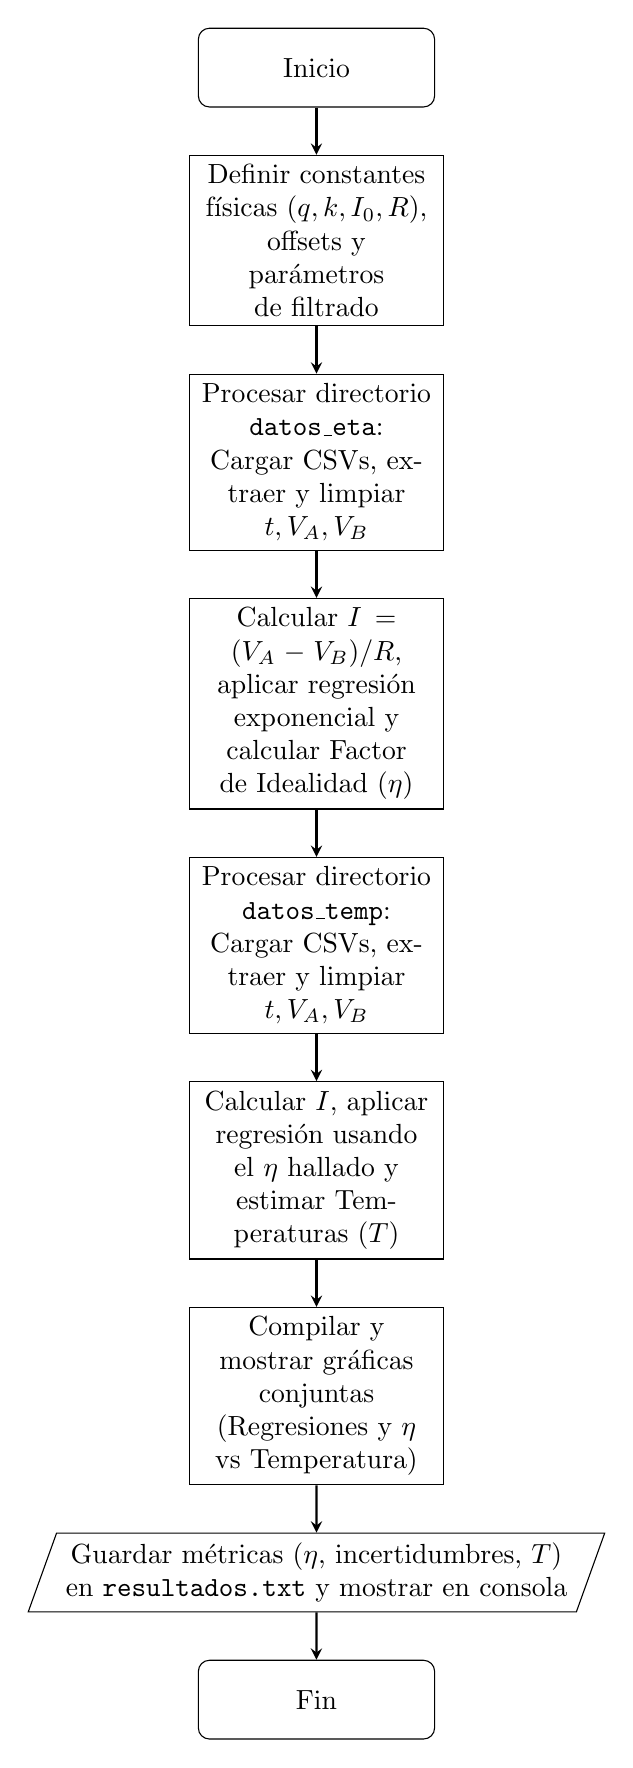
\begin{tikzpicture}[node distance=0.6cm, auto]
        
        % --- Definición de nodos ---
        \node (start) [startstop] {Inicio};
        
        \node (init) [process, below=of start, align=center] {Definir constantes físicas ($q, k, I_0, R$), \\ offsets y parámetros de filtrado};
        
        \node (eta_data) [process, below=of init, align=center] {Procesar directorio \texttt{datos\_eta}: \\ Cargar CSVs, extraer y limpiar $t, V_A, V_B$};
        
        \node (eta_calc) [process, below=of eta_data, align=center] {Calcular $I = (V_A - V_B) / R$, aplicar regresión \\ exponencial y calcular Factor de Idealidad ($\eta$)};
        
        \node (temp_data) [process, below=of eta_calc, align=center] {Procesar directorio \texttt{datos\_temp}: \\ Cargar CSVs, extraer y limpiar $t, V_A, V_B$};
        
        \node (temp_calc) [process, below=of temp_data, align=center] {Calcular $I$, aplicar regresión usando \\ el $\eta$ hallado y estimar Temperaturas ($T$)};
        
        \node (plots) [process, below=of temp_calc, align=center] {Compilar y mostrar gráficas conjuntas \\ (Regresiones y $\eta$ vs Temperatura)};
        
        \node (save) [io, below=of plots, align=center] {Guardar métricas ($\eta$, incertidumbres, $T$) \\ en \texttt{resultados.txt} y mostrar en consola};
        
        \node (stop) [startstop, below=of save] {Fin};

        % --- Conexiones ---
        \draw [arrow] (start) -- (init);
        \draw [arrow] (init) -- (eta_data);
        \draw [arrow] (eta_data) -- (eta_calc);
        \draw [arrow] (eta_calc) -- (temp_data);
        \draw [arrow] (temp_data) -- (temp_calc);
        \draw [arrow] (temp_calc) -- (plots);
        \draw [arrow] (plots) -- (save);
        \draw [arrow] (save) -- (stop);

    \end{tikzpicture}
    }
    \caption{Diagrama de flujo del script principal para el análisis y procesamiento de los datos (\texttt{main.py}).}
    \label{fig:flow_main_python}
\end{figure}

\section{Análisis de Resultados}
\label{sec:resultados}

En esta sección se presentan y discuten los datos adquiridos experimentalmente y los parámetros calculados mediante los algoritmos de regresión. El análisis se divide en la evaluación temporal de las señales, la extracción empírica del factor de idealidad y la validación del modelo de estimación térmica.

\subsection{Análisis de la Adquisición de Señales}
Para garantizar una alta resolución en la captura de transitorios y evitar pérdidas de información en la zona de conducción del diodo, el sistema se configuró para adquirir \num{5000} muestras a lo largo de dos periodos de una señal de excitación de \SI{1}{\hertz}. Esto corresponde a una ventana de captura total de \SI{2}{\second} con un periodo de muestreo efectivo de \SI{400}{\micro\second}.

En la Fig. \ref{fig:sim_montaje} se presenta la implementación en simulación del sistema de adquisición de datos, destacando el circuito de acondicionamiento y el diodo bajo prueba con su respectivas gráficas de salida.

\begin{figure}[H]
    \centering
    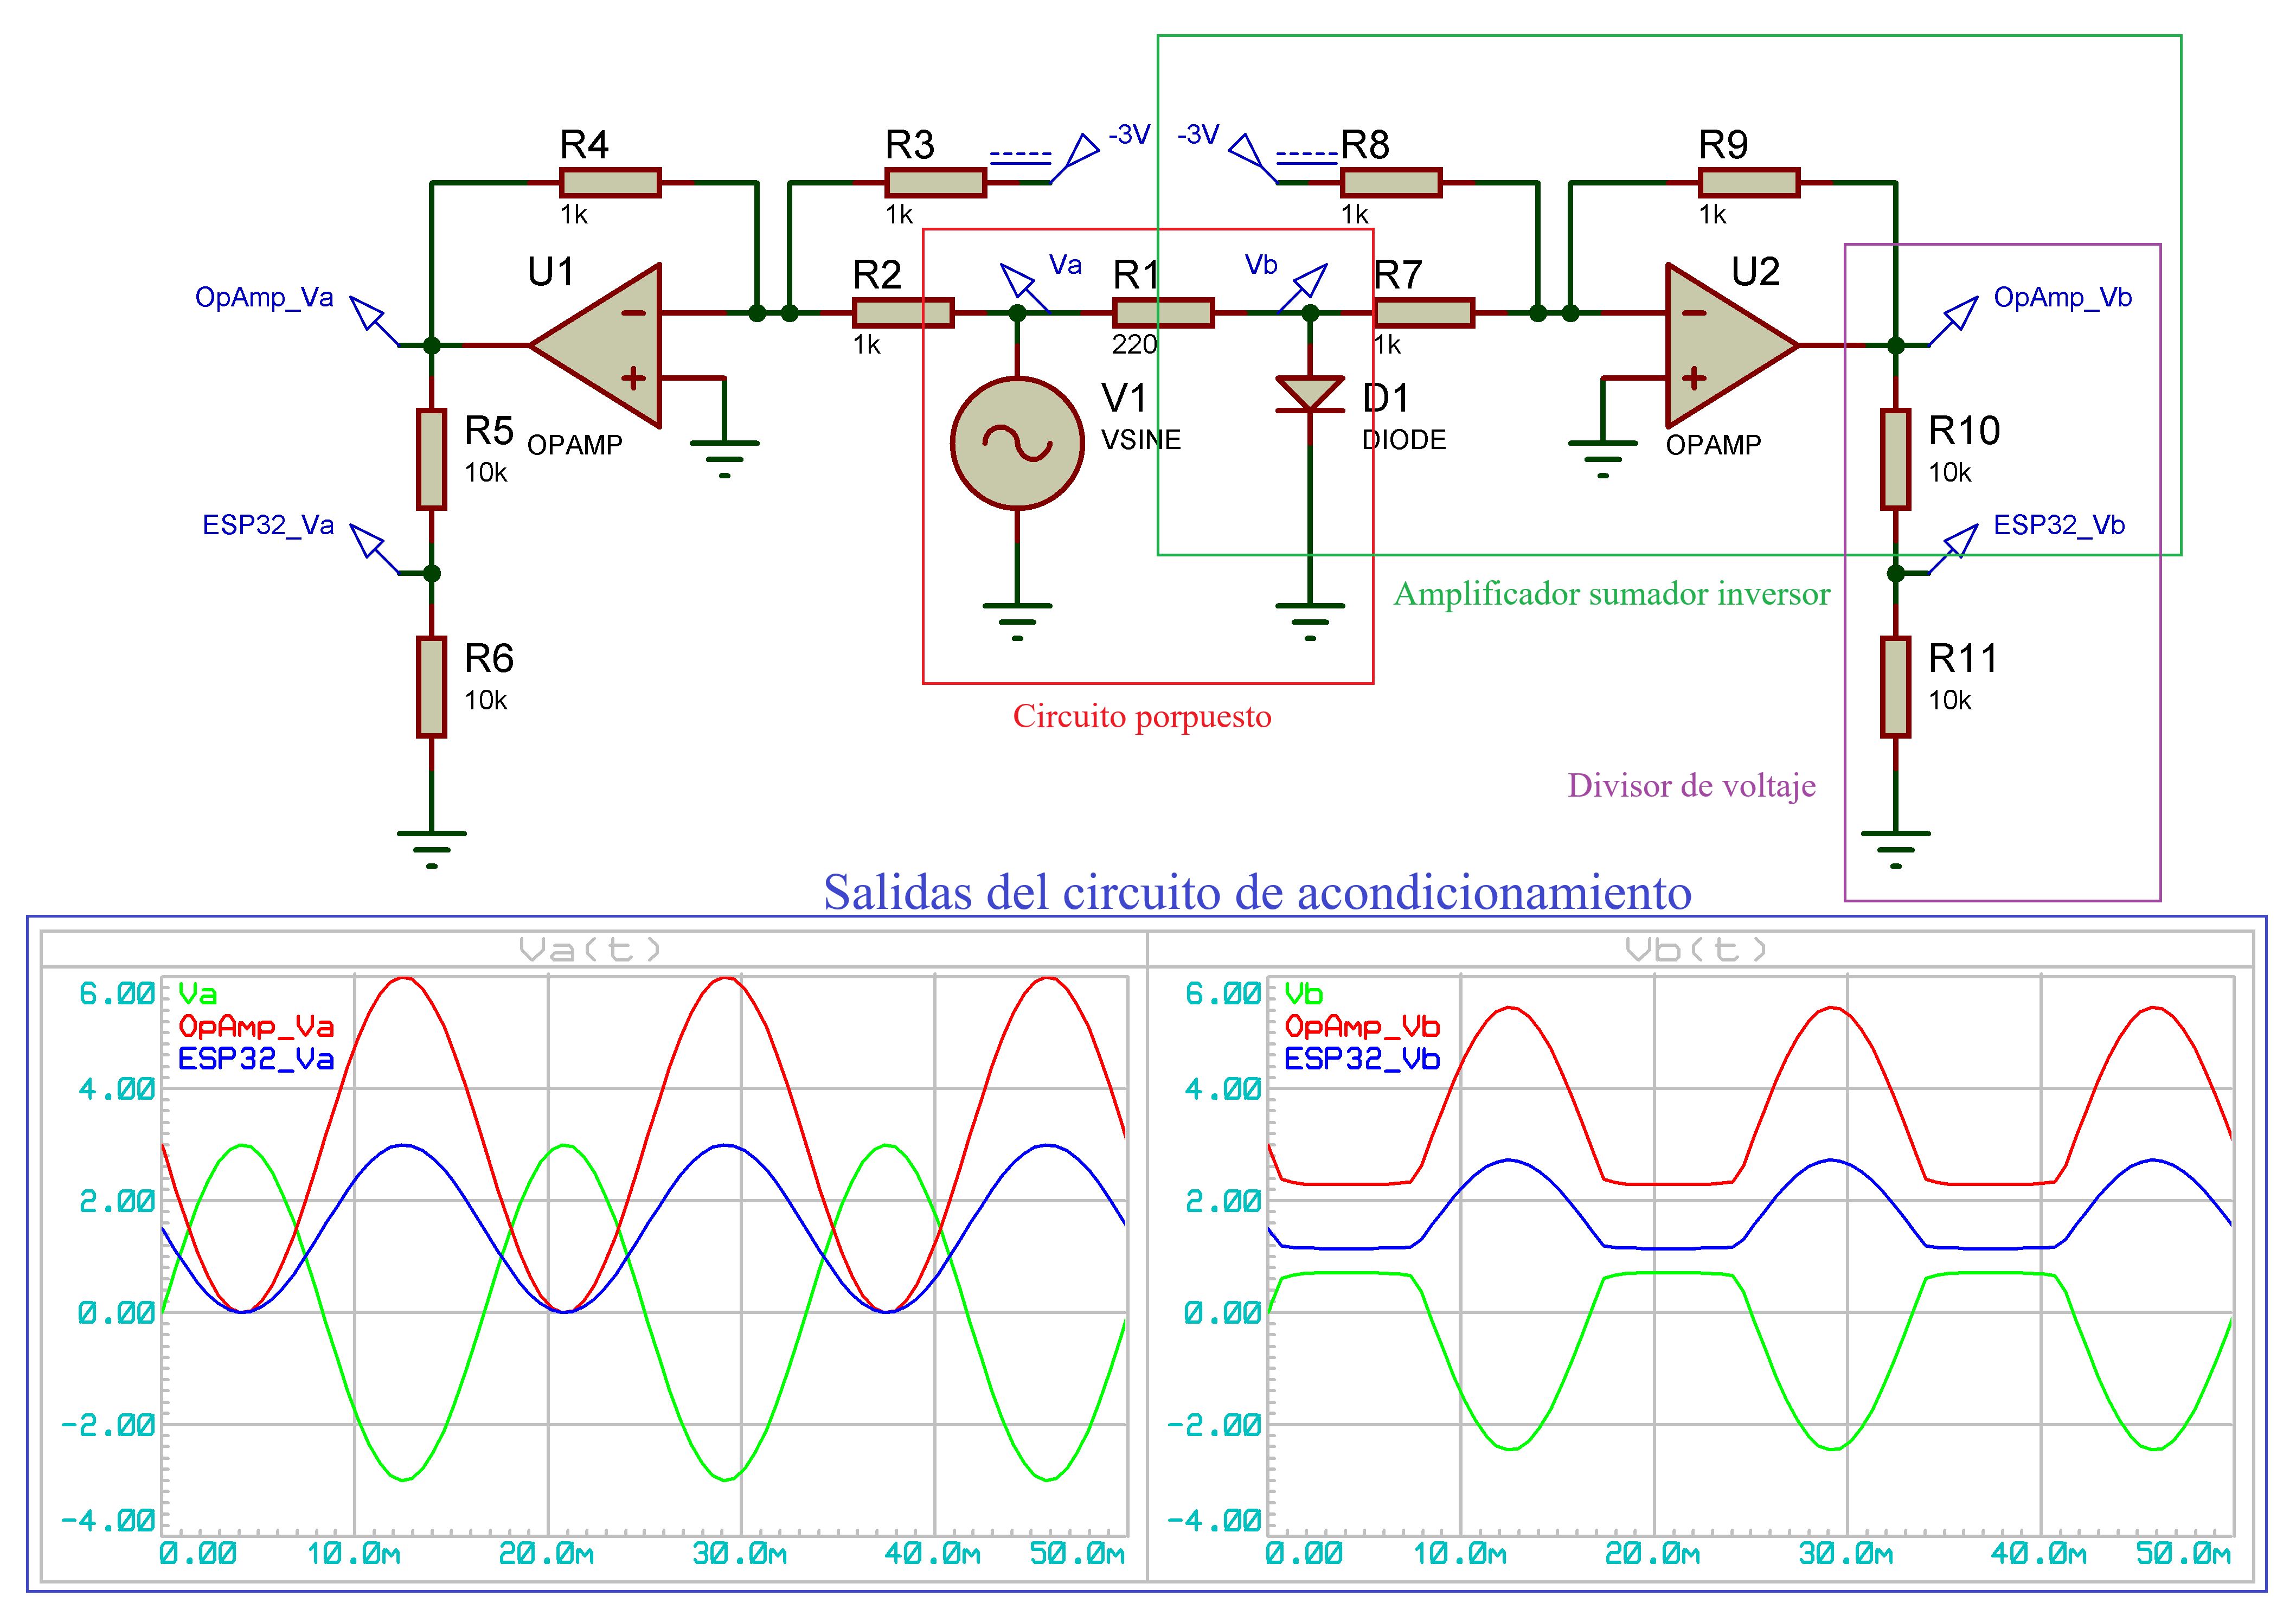
\includegraphics[width=\columnwidth]{sim_circuito.png}
    \caption{Simulación de la configuración del hardware y conexionado del sistema DAQ.}
    \label{fig:sim_montaje}
\end{figure}

Las formas de onda digitalizadas se presentan en la Fig. \ref{fig:grafica_voltajes}. La señal del nodo $V_A$ describe la onda senoidal pura suministrada por el generador, mientras que la señal $V_B$ (tensión sobre el diodo) exhibe un claro recorte (achatamiento) durante el semiciclo positivo. Este comportamiento evidencia físicamente el instante en que el diodo supera su barrera de potencial y entra en polarización directa, limitando el crecimiento del voltaje en sus terminales.

\begin{figure}[htbp]
    \centering
    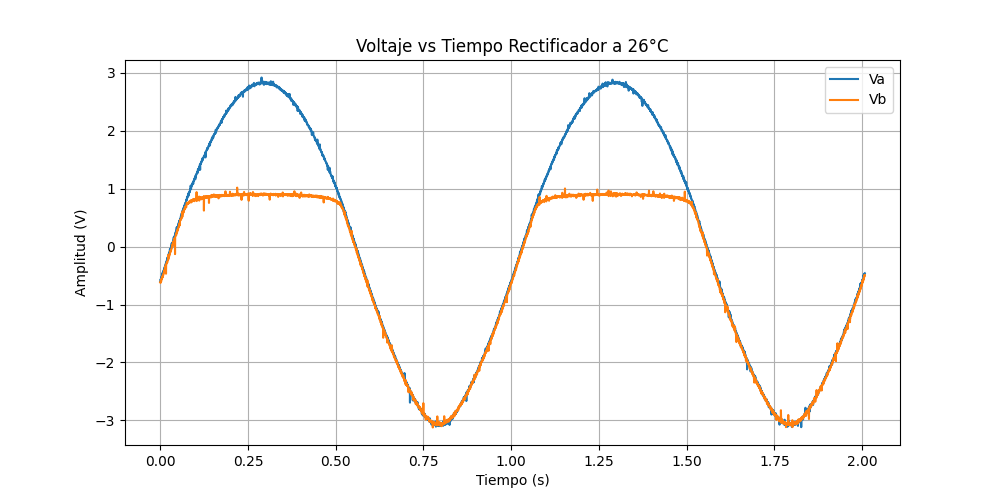
\includegraphics[width=\columnwidth]{grafica_voltajes.png}
    \caption{Señales de voltaje adquiridas simultáneamente por los canales ADC de la ESP32 ($V_A$ y $V_B$) a una frecuencia de \SI{1}{\hertz}.}
    \label{fig:grafica_voltajes}
\end{figure}

A partir de la diferencia de potencial ($V_A - V_B$) y el valor de la resistencia serie, se calculó la corriente instantánea del circuito (Fig. \ref{fig:grafica_corriente}). La gráfica demuestra que la conducción ocurre exclusivamente durante la fase activa del voltaje, con una ausencia de desfase que valida la naturaleza resistiva del sistema de medición.

\begin{figure}[htbp]
    \centering
    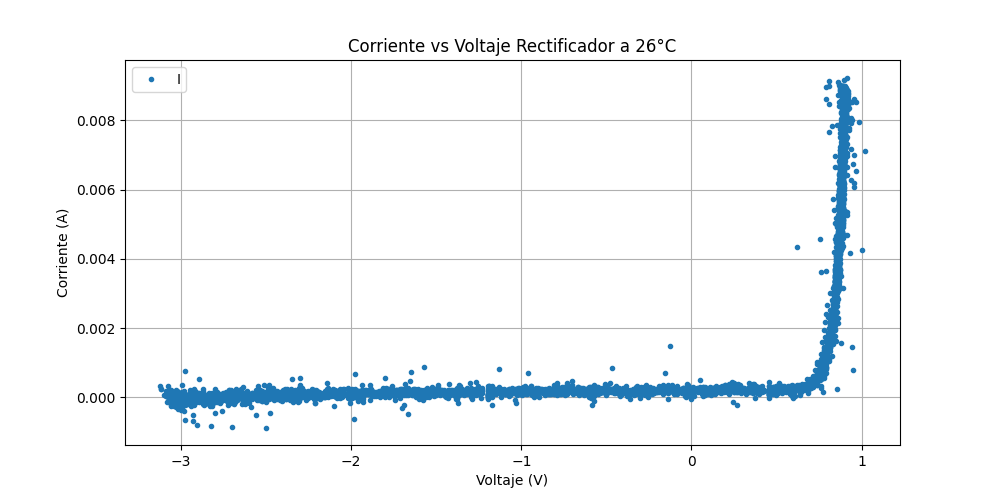
\includegraphics[width=\columnwidth]{grafica_corriente.png}
    \caption{Corriente instantánea calculada a través del diodo ($i_D$) mostrando los ciclos de conducción y bloqueo.}
    \label{fig:grafica_corriente}
\end{figure}

\subsection{Caracterización del Factor de Idealidad ($\eta$)}
El primer ajuste algorítmico se aplicó sobre los datos capturados a temperatura ambiente ($T = \SI{299.15}{\kelvin}$ o \SI{26}{\celsius}). En la Fig. \ref{fig:grafica_regresion} se ilustra la superposición entre los puntos experimentales dispersos y el modelo matemático optimizado mediante el algoritmo de Levenberg-Marquardt. 

\begin{figure}[htbp]
    \centering
    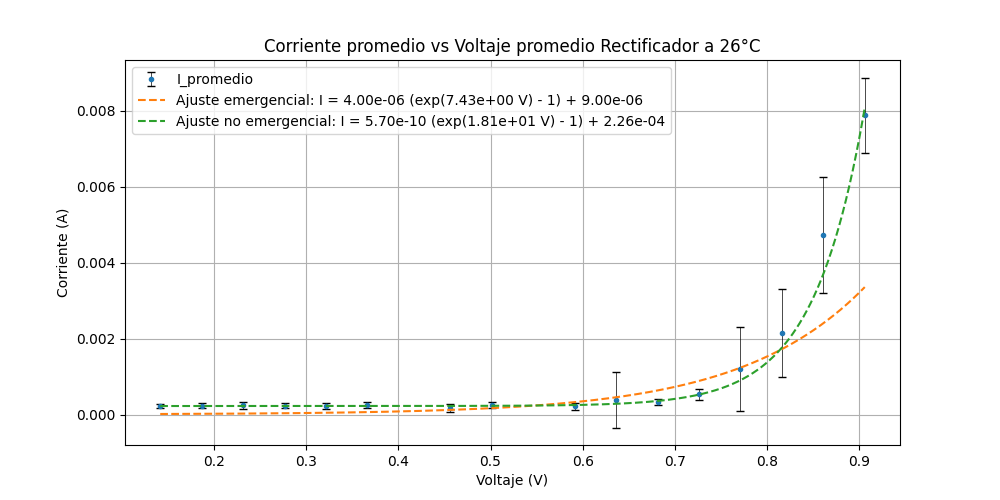
\includegraphics[width=\columnwidth]{grafica_regresion.png}
    \caption{Curva $V-I$ a temperatura ambiente comparada con el ajuste no lineal del modelo de Shockley.}
    \label{fig:grafica_regresion}
\end{figure}

Como se resumirá posteriormente en la Tabla \ref{tab:resultados_eta}, la regresión arrojó un factor de idealidad de $\eta \approx 2.138$, con una incertidumbre propagada de $\pm 0.247$. La ecuación característica extraída para este estado fue:
\begin{equation}
    I = \num{5.70e-10} \left( \exp \left({\num{1.81e01} V}\right) - 1 \right) + \num{2.26e-04}
\end{equation}

\begin{table}[htbp]
\caption{Parámetros extraídos para la caracterización del factor de idealidad ($\eta$) a temperatura ambiente ($26^\circ$C).}
\begin{center}
\begin{tabular}{|c|c|c|}
\hline
\makecell{Parámetro} & \makecell{Valor Calculado} & \makecell{Incertidumbre ($\pm$)}\\
\hline
Factor de idealidad ($\eta$) & $2.138$ & $0.247$ \\
Coeficiente de saturación $A$ (A) & $5.70 \times 10^{-10}$ & N/A \\
Término de compensación $C$ (A) & $2.26 \times 10^{-4}$ & N/A \\
Coeficiente exponencial $B$ & $18.10$ & N/A \\
\hline
\end{tabular}
\label{tab:resultados_eta}
\end{center}
\end{table}


Físicamente, un valor de $\eta > 2$ indica que, en el dispositivo bajo prueba, los fenómenos de recombinación de portadores en la región de agotamiento (space-charge region) tienen un peso considerable frente a la corriente de difusión pura, lo cual es un comportamiento típico en diodos rectificadores no ideales. La inclusión del término de compensación $C = \num{2.26e-04}$ fue clave para absorber las no linealidades originadas por la resistencia en serie del material y las corrientes de fuga instrumentales, logrando un ajuste con alta fidelidad visual en la zona exponencial.

\begin{figure}[htbp]
    \centering
    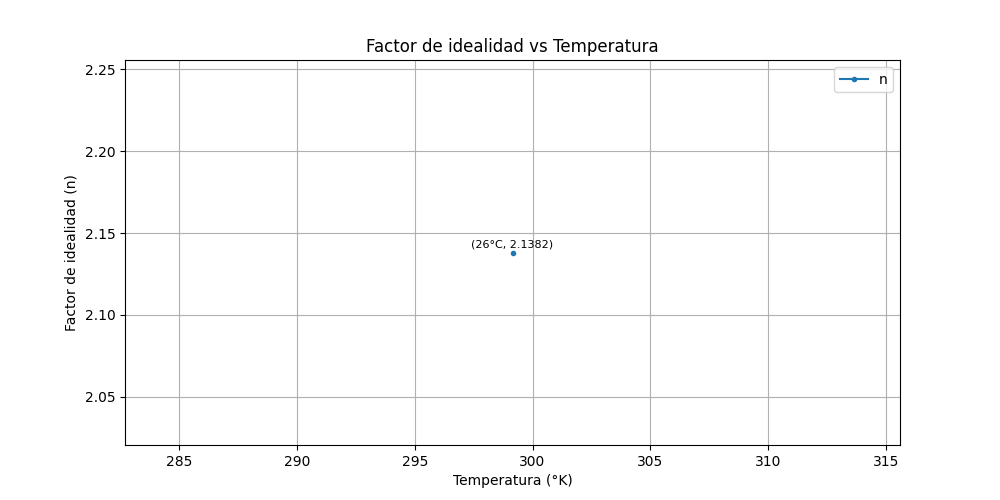
\includegraphics[width=0.45\textwidth]{grafica_factor_idealidad.png}
    \caption{Representación gráfica de la extracción del factor de idealidad ($\eta$) y su margen de incertidumbre.}
    \label{fig:grafica_factor_idealidad}
\end{figure}

\subsection{Análisis de la Sensibilidad Térmica y Estimación de T}
Una vez fijado el parámetro estructural $\eta$, se evaluó la respuesta térmica del diodo aplicando una temperatura controlada de \SI{100}{\celsius} (\SI{373.15}{\kelvin}). Como se aprecia en la Fig. \ref{fig:grafica_regresiones_temperaturas}, el aumento de energía térmica genera un desplazamiento evidente de la curva de conducción hacia la izquierda. Este fenómeno ocurre porque la energía térmica intrínseca facilita a los electrones superar la barrera de potencial, requiriendo un menor voltaje de polarización directa para alcanzar el mismo nivel de corriente.

\begin{figure}[htbp]
    \centering
    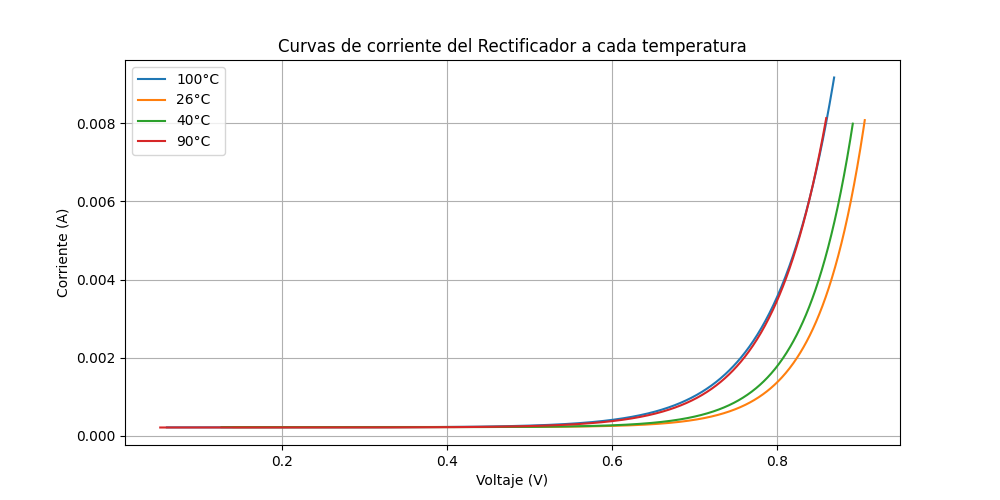
\includegraphics[width=0.45\textwidth]{grafica_regresiones_temperaturas.png}
    \caption{Comparación de las curvas de regresión ajustadas para los datos a temperatura ambiente (\SI{26}{\celsius}) y estado de calentamiento.}
    \label{fig:grafica_regresiones_temperaturas}
\end{figure}

El algoritmo de estimación utilizó los datos del escenario de calentamiento para despejar la temperatura real de la unión ($T$). Según los datos recopilados en la Tabla \ref{tab:resultados_temp}, el modelo estimó una temperatura de $T \approx \SI{379.81}{\kelvin}$ (\SI{106.66}{\celsius}), con un margen de incertidumbre estadística de $\pm \SI{45.48}{\kelvin}$. La ecuación del ajuste térmico resultó ser:
\begin{equation}
    I = \num{3.62e-08} \left( \exp \left({\num{1.43e01} V}\right) - 1 \right) + \num{2.19e-04}
\end{equation}

\begin{table}[htbp]
\caption{Comparativa entre las temperaturas nominales de ensayo y las estimaciones calculadas por el modelo.}
\begin{center}
\begin{tabular}{|c|c|c|c|}
\hline
\makecell{T Nominal\\($^\circ$C)} & \makecell{T Estimada\\($^\circ$C)} & \makecell{Incertidumbre\\($\pm$ $^\circ$C)} & \makecell{Error Relativo\\(\%)}\\
\hline
$26.00^\circ$C & $26.00^\circ$C & $34.55$ & $0.00\%$ \\
$40.00^\circ$C & $36.50^\circ$C & $41.10$ & $8.75\%$ \\
$90.00^\circ$C & $89.30^\circ$C & $55.98$ & $0.78\%$ \\
$100.00^\circ$C & $106.66^\circ$C & $45.48$ & $6.66\%$ \\
\hline
\end{tabular}
\label{tab:resultados_temp}
\end{center}
\end{table}

El valor calculado presenta un error relativo del $6.6\%$ respecto al valor nominal de excitación térmica (\SI{100}{\celsius}). Matemáticamente, este error se propaga a través de la sensibilidad exponencial del parámetro de ajuste $B$. Desde el punto de vista físico, la desviación se justifica por el gradiente de temperatura existente entre la fuente externa de calor y la unión interna real del semiconductor. Además, el modelo asume a $\eta$ como una constante estrictamente invariante; sin embargo, en regímenes de alta temperatura, la sección transversal de captura para la recombinación varía ligeramente, introduciendo pequeñas perturbaciones en el cálculo final. A pesar de esto, el algoritmo demuestra la capacidad de traducir el corrimiento de la curva $V-I$ en una medición termométrica altamente coherente.

\section{Conclusiones}

El sistema de adquisición de datos implementado, basado en el microcontrolador ESP32 y su respectiva etapa de acondicionamiento analógico, demostró ser altamente efectivo para la captura de la dinámica no lineal del dispositivo semiconductor. La aplicación del algoritmo de optimización de Levenberg-Marquardt permitió un ajuste robusto de los datos experimentales al modelo de la ecuación de Shockley, logrando extraer un factor de idealidad coherente con la naturaleza del componente. El valor obtenido confirma que en este tipo de rectificadores predominan los fenómenos de recombinación en la región de agotamiento por encima de la difusión ideal.

Por otro lado, la inversión del modelo matemático validó la viabilidad empírica de utilizar el diodo como un sensor de temperatura. El corrimiento de la curva de voltaje y corriente hacia la izquierda comprobó físicamente que el incremento en la energía térmica de los portadores facilita la conducción a menores voltajes. Las estimaciones térmicas arrojaron una alta fidelidad a lo largo de las pruebas, destacando un desempeño sobresaliente y un error relativo inferior al uno por ciento en la región cercana a los noventa grados Celsius.

Finalmente, las divergencias encontradas en los extremos térmicos de prueba se justifican por la presencia de gradientes de temperatura entre la unión interna del dispositivo y la fuente de calor externa, sumado a la pequeña variación intrínseca del factor de idealidad que el modelo base asume como constante. A pesar de estas consideraciones físicas, la metodología integral de hardware y software propuesta establece un marco de trabajo preciso, automatizado y de bajo costo para la caracterización termoelectrónica de diodos.

\bibliographystyle{IEEEtran}
\bibliography{IEEEabrv,biblio_traps_dynamics}

\end{document}